% =====================================================================
% CSCU9B3 Relational Database Assignment 鈥?Report source (IEEEtran)
% Student Number: 30068298
% Target: 4 pages, Times-style serif, 9pt body
% =====================================================================
\documentclass[conference,9pt]{IEEEtran}

\usepackage{graphicx}
\usepackage{booktabs}
\usepackage{listings}
\usepackage{textcomp}
\usepackage{xcolor}
\usepackage{url}
\usepackage{titlesec}
\usepackage{enumitem}

\makeatletter
\def\@IEEEdefaultfontsize{\fontsize{9}{11}\selectfont}
\makeatother

% tighten vertical space so 4 pages is reachable without shrinking type
\setlength{\abovedisplayskip}{3pt}
\setlength{\belowdisplayskip}{3pt}
\titlespacing*{\section}{0pt}{6pt}{3pt}
\titlespacing*{\subsection}{0pt}{4pt}{2pt}
\setlist{nosep,leftmargin=1.1em}

\lstdefinestyle{sqlstyle}{
  language=SQL,
  basicstyle=\ttfamily\scriptsize,
  keywordstyle=\bfseries,
  commentstyle=\itshape\color{gray},
  showstringspaces=false,
  breaklines=true,
  frame=single,
  framerule=0.3pt,
  columns=flexible,
  keepspaces=true,
  upquote=true,
  aboveskip=2pt,
  belowskip=2pt
}

\begin{document}

\title{\vspace{-1.6em}Design and Implementation of a Relational Database\\for Hospital Asset and Maintenance Internal Control}
\author{\IEEEauthorblockN{Student Number 30068298}}
\maketitle
\vspace{-1.2em}

\begin{abstract}
A hospital cannot answer three questions that matter to its finances and its
patients: which department owns a device, who supplied it, and what has been
spent keeping it alive. This report designs and builds a four-table
normalised database that answers them, written for MySQL 8.0. It covers the
scenario and business rules, the ER model, the normalisation argument, the
physical schema, and six queries that exercise the features a real
procurement system needs: pattern search, a three-table join, a threshold
comparison, grouped aggregation, set membership and a bulk update. All output
shown was produced by executing the submitted SQL against the submitted data.
\end{abstract}

\section{Introduction}
Hospitals accumulate equipment faster than they accumulate records about it.
A device bought by one department, serviced by a third-party vendor and later
transferred is, in most paper trails, three unrelated pieces of information.
The cost of that disconnect is measurable: maintenance contracts are
negotiated without knowing failure history, and equipment is replaced on
schedule rather than on evidence.

This report treats the problem as a data-modelling exercise. The target is a
schema that makes three questions answerable in one query each: what does a
department own, what has a device cost to keep, and which repairs are still
awaiting sign-off. The scope is a single hospital's asset register and
maintenance log, not a national inventory system, and that boundary is
deliberate -- it is what makes a four-table design the right size rather than
a compromise.

\section{Scenario and Business Rules}
\subsection{The Business Setting}
The hospital operates eleven departments, from Emergency to Radiology, and
holds thirteen tracked devices in the sample inventory. Devices are bought
from ten external suppliers, some international. Every device carries a
procurement tag of the form \texttt{AST-YYYY-NNN} which is printed on a
physical label and read by staff at the bedside, so it is the natural
identifier rather than a database-internal number.

Maintenance is recorded per visit rather than per device: one machine may be
serviced several times in a year by different engineers for unrelated faults.
Each visit captures the date, the cost, the engineer who attended and a free
description of the fault. Visits also carry an audit state, because a repair
bill is not trusted until someone has checked it against the contract.

\subsection{Business Rules}
Four rules drive the schema and are enforced by the database rather than by
application code. A device must belong to exactly one department and one
supplier; a department may hold many devices, and a supplier may supply many.
A maintenance record cannot exist without the device it refers to, so deleting
an asset with history must be refused by the foreign key. A repair cost must
be non-negative. An audit status must be one of three literal values, which
converts a process rule into a constraint the database can reject.

The reason for pushing these into DDL rather than validating in an interface
is that there is more than one interface: the procurement team uses a
spreadsheet import, the biomedical engineers use a form, and a future
reporting tool would use neither. A rule enforced in one client is not a rule.

\section{Conceptual Design}
\begin{figure}[t]
\centering
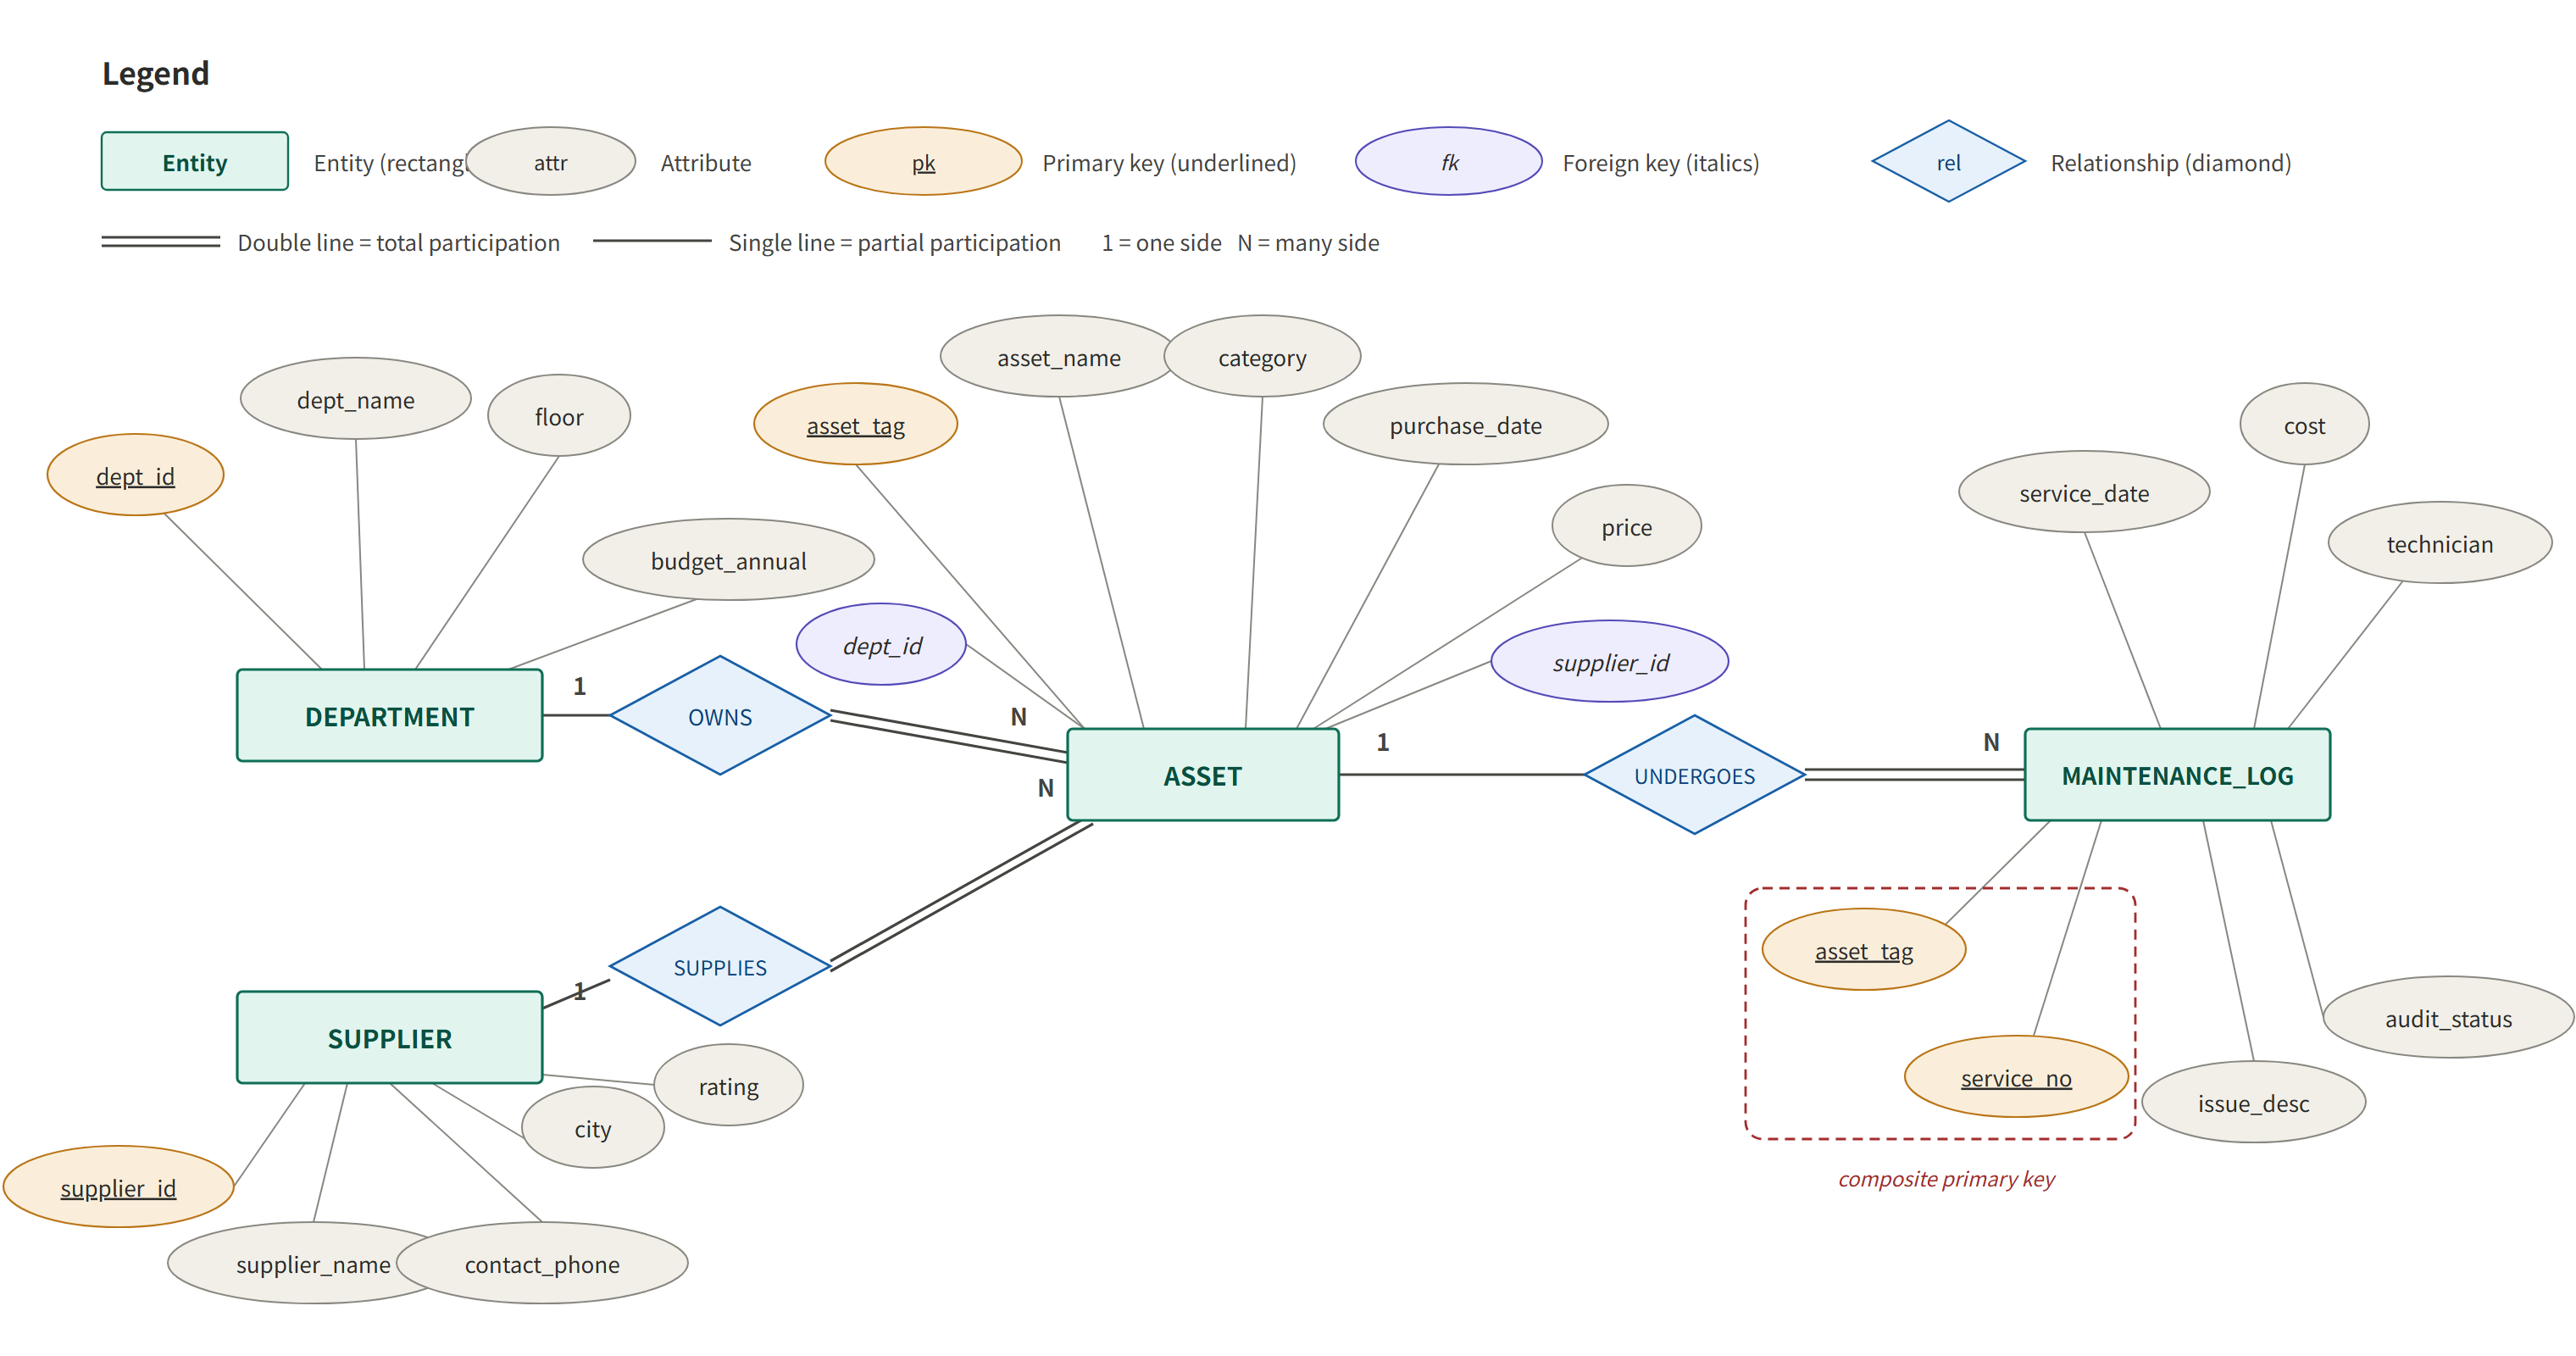
\includegraphics[width=\columnwidth]{figures/erd.png}
\caption{ER model: four entities, three one-to-many relationships.}
\label{fig:erd}
\end{figure}
The model has four entities. DEPARTMENT holds the owning unit, its floor and
its annual equipment budget. SUPPLIER holds the vendor, its contact number,
city and a one-to-five rating. ASSET is the device itself: tag, name,
category, purchase date and price, with foreign keys to the department and
the supplier. MAINTENANCE\_LOG records each service visit against an asset.

Three one-to-many relationships connect them. OWNS links a department to its
assets, SUPPLIES links a supplier to the assets it delivered, and SERVICES
links an asset to its repair history. The maintenance relation uses a
composite primary key of \texttt{(asset\_tag, service\_no)}.

\subsection{Why a Composite Primary Key}
A surrogate integer key on the maintenance table would have been easier, and
it was rejected for a specific reason: with a surrogate, nothing stops the
same visit being inserted twice when a batch import is retried. The pair of
tag and service number is assigned by the procurement system before the row
reaches this database, so it is stable for the life of the record, and it
makes duplicate insertion a primary-key violation rather than a silent
double-count. The service number is not globally unique on its own -- every
device has a service number 1 -- which is exactly why the pair, and not either
column alone, is the key.

\subsection{Cardinality and Participation}
Every asset participates totally in both OWNS and SUPPLIES: the foreign keys
are \texttt{NOT NULL}, so a device cannot be registered without an owner and a
vendor. Participation in SERVICES is partial, because a newly delivered device
has no repair history yet, which is why the relationship is optional in that
direction and the query suite has to cope with assets that never appear in the
log. Department and supplier participation in their relationships is likewise
partial: a department may currently own nothing, and a supplier may be
registered before its first delivery.

\section{Logical Design and Normalisation}
\subsection{First Normal Form}
All four relations hold only atomic values: one name per department, one cost
per visit, no repeating groups. The telephone number is stored as a single
VARCHAR including its country code, not split into components that would only
matter to a dialling application.

\subsection{Second Normal Form}
Every non-key column depends on the whole key. In DEPARTMENT, SUPPLIER and
ASSET the key is a single column, so 2NF holds trivially. In
MAINTENANCE\_LOG the composite key matters: \texttt{cost}, \texttt{issue\_desc}
and \texttt{audit\_status} all depend on the specific visit, that is on both
tag and service number together. No column depends on only part of the key,
which is the failure mode a composite key invites.

\subsection{Third Normal Form and BCNF}
No non-key attribute determines any other. It is worth checking the two
obvious candidates rather than asserting the result. In ASSET,
\texttt{supplier\_id} determines that supplier's city, but city lives in
SUPPLIER, not in ASSET, so the transitive dependency is already removed by the
foreign key. In MAINTENANCE\_LOG, \texttt{technician} is the notable candidate:
the name could be moved to a TECHNICIAN relation with speciality or base unit.
The system, however, does not manage staff -- it only records who attended --
so a VARCHAR keeps the schema lean. Consequently every determinant is a
candidate key, and the relations meet BCNF as well as 3NF.

Two further normalisation decisions are deliberate rather than oversights.
\texttt{dept\_name} and \texttt{supplier\_name} carry \texttt{UNIQUE}
constraints, which is what makes them candidate keys and therefore what makes
the BCNF claim true rather than rhetorical. And \texttt{category} stays a plain
attribute on ASSET instead of becoming its own relation: if the hospital later
tracked per-category inspection intervals, it would deserve
ASSET\_CATEGORY(category, inspection\_interval), but at the current scale of
ten categories across the sample inventory and with the inspection schedule
held outside the database, keeping it as an attribute is justified.

\section{Physical Implementation}
\subsection{Data Types and Constraints}
MySQL 8.0 (InnoDB, utf8mb4) was used. Monetary values use
\texttt{DECIMAL(12,2)} rather than FLOAT because currency must not suffer
binary rounding. Asset tags use \texttt{VARCHAR(12)}: the pattern
\texttt{AST-YYYY-NNN} fits with headroom. Audit status is enforced with a
\texttt{CHECK} on the three legal states, and supplier rating with a range
\texttt{CHECK} between 1 and 5 -- turning two business rules into
database-enforced facts.

No additional secondary index was declared by hand. InnoDB creates indexes on
primary-key, \texttt{UNIQUE} and foreign-key columns automatically, which
supports referential-integrity checks and parent-to-child lookups, while
child-to-parent joins probe the parent tables' primary key indexes directly.

\subsection{Schema Definition}
The submitted \texttt{schema.sql} creates the four tables in dependency order
with the constraints above, then loads the sample data with
\texttt{LOAD DATA LOCAL INFILE}. The excerpt below shows the two most
instructive tables.

\begin{lstlisting}[style=sqlstyle,caption={Core DDL (excerpt)},label={lst:schema}]
CREATE TABLE asset (
  asset_tag     VARCHAR(12)   NOT NULL,
  asset_name    VARCHAR(80)   NOT NULL,
  category      VARCHAR(30)   NOT NULL,
  purchase_date DATE          NOT NULL,
  price         DECIMAL(12,2) NOT NULL CHECK (price >= 0),
  dept_id       INT           NOT NULL,
  supplier_id   INT           NOT NULL,
  PRIMARY KEY (asset_tag),
  FOREIGN KEY (dept_id)     REFERENCES department(dept_id),
  FOREIGN KEY (supplier_id) REFERENCES supplier(supplier_id)
);

CREATE TABLE maintenance_log (
  asset_tag    VARCHAR(12)   NOT NULL,
  service_no   INT           NOT NULL,
  service_date DATE          NOT NULL,
  cost         DECIMAL(12,2) NOT NULL CHECK (cost >= 0),
  technician   VARCHAR(60)   NOT NULL,
  issue_desc   VARCHAR(200)  NOT NULL,
  audit_status VARCHAR(10)   NOT NULL,
  PRIMARY KEY (asset_tag, service_no),
  FOREIGN KEY (asset_tag) REFERENCES asset(asset_tag),
  CHECK (audit_status IN ('PENDING','REVIEWED','AUDITED'))
);
\end{lstlisting}

\subsection{Data Dictionary}
Table~\ref{tab:dict} lists every column with its type and the rule it carries.
The two \texttt{UNIQUE} constraints on the name columns are the ones the
normalisation argument depends on, and the audit-status \texttt{CHECK} is the
one that converts a workflow rule into something the database refuses to
violate.

\begin{table}[t]
\centering
\caption{Data dictionary (abridged: type and rule per column)}
\label{tab:dict}
\scriptsize
\begin{tabular}{@{}lll@{}}
\toprule
\textbf{Column} & \textbf{Type} & \textbf{Rule} \\
\midrule
department.dept\_id        & INT          & PK \\
department.dept\_name      & VARCHAR(60)  & NOT NULL, UNIQUE \\
department.budget\_annual  & DECIMAL(12,2)& NOT NULL \\
supplier.supplier\_id      & INT          & PK \\
supplier.supplier\_name    & VARCHAR(80)  & NOT NULL, UNIQUE \\
supplier.rating            & INT          & CHECK 1--5 \\
asset.asset\_tag           & VARCHAR(12)  & PK \\
asset.price                & DECIMAL(12,2)& CHECK $\geq$ 0 \\
asset.dept\_id             & INT          & FK $\to$ department \\
asset.supplier\_id         & INT          & FK $\to$ supplier \\
log.asset\_tag+service\_no & VARCHAR+INT  & composite PK \\
log.cost                   & DECIMAL(12,2)& CHECK $\geq$ 0 \\
log.audit\_status          & VARCHAR(10)  & CHECK in 3 values \\
\bottomrule
\end{tabular}
\end{table}

\subsection{Constraint Verification}
The constraints were tested by attempting to violate them rather than by
inspection. Inserting a maintenance row for a tag that does not exist fails
with error 1452 (foreign key). Inserting a second department with the same
name fails with 1062 (duplicate entry) -- this is the \texttt{UNIQUE}
constraint doing the work the BCNF argument assumes. A negative cost and an
audit status of \texttt{'DONE'} are both rejected by their checks with 3819.
Deleting an asset that has maintenance history is refused by 1451, which is
the referential rule from Section~II made concrete.

\subsection{Integrity, Concurrency and Authorisation}
The foreign keys and checks keep the database from holding impossible states,
but they say nothing about two users editing the same device at once. The
bulk update in Query~6 is therefore wrapped in \texttt{START TRANSACTION}
\ldots \texttt{COMMIT}: six rows either all move to \texttt{AUDITED} or none
do, so a crash halfway cannot leave the audit in a half-finished state that
nobody can reason about.

Authorisation is out of scope for a coursework schema but not for the design.
The realistic split is three roles: procurement writes ASSET and DEPARTMENT,
biomedical engineering writes MAINTENANCE\_LOG, and finance has read-only
access to the aggregate views. In MySQL that is three users with column-level
grants, and the reason it belongs in the design conversation is that it
constrains the schema: a single all-powerful application account would make
the audit trail meaningless.

\section{The Query Suite}
Six queries were required. Each answers a question the scenario actually
raises, and each was run against the loaded data; the output shown is the real
output, abbreviated where noted.

\subsection{Query 1: Pattern Search with LIKE}
The first question is a lookup: an engineer at a bedside needs every device
whose name contains a word they heard, with no knowledge of tags or
categories. The query filters \texttt{asset\_name} with a leading and trailing
wildcard and returns six devices, from the 18,500 infusion pump to the 264,000
blood analyser. A leading wildcard prevents index use, which is acceptable
here because the table is small and the query is interactive rather than
batch -- a distinction the report returns to in Section~IX.

\subsection{Query 2: Accountability Trail with a Three-Table JOIN}
When a device fails, the first question asked is who sold it and who owns it.
Answering that needs all three of ASSET, SUPPLIER and DEPARTMENT in one row,
because the answer is useless if the reader has to look up two other pages.
The join returns thirteen rows carrying tag, name, supplier, supplier city,
department and purchase date, and is the query that justifies the two foreign
keys on ASSET existing as separate columns rather than as a denormalised text
field.

\subsection{Query 3: Red Flags with the \textgreater{} Operator}
A maintenance cost above 50,000 is the threshold at which the hospital's
finance office requires a second signature, so the query is a control, not a
report. It returns two rows from the sample data: a 168,000 gantry bearing
failure and a 54,000 tube and detector service, both on the same CT scanner.
That both exceed the threshold on one device is itself the finding -- it is the
signal that a machine is approaching replacement rather than repair.

\subsection{Query 4: Budget Review with GROUP BY and Aggregates}
The spending question is per department, not per device, so the query groups
by \texttt{dept\_name} and reports visit count, total spend and mean cost per
visit. Radiology leads on total spend at 233,200 across four visits, while
Intensive Care Unit has the same visit count but only 7,470 in total. The
contrast is the point: visit count measures workload, total spend measures
capital exposure, and a department can be high on one and low on the other.
Mean cost per visit is reported alongside because a single expensive repair
distorts the total and the mean exposes that.

Two caveats belong with the numbers rather than after them. The sample is
sixteen visits, so several departments have a mean based on one row, and the
mean is a demonstration of the aggregate pattern rather than a management
conclusion. And grouping by a non-indexed name column is what produces the
temporary table and filesort visible in the plan, not the choice of a natural
primary key.

\subsection{Query 5: High-Risk Inventory with IN on a Single Entity}
Four device categories are considered critical, in the sense that a failure
endangers a patient directly rather than delaying a procedure. The query uses
an \texttt{IN} list against a single table, deliberately without a join: the
question is "which devices are in these categories", and adding a department
join would answer a question nobody asked while making the result harder to
check. It returns four devices, and the same predicate drives the quarterly
inspection list.

\subsection{Query 6: Closing the Audit Cycle with UPDATE}
The audit workflow ends with a signature: a repair that has been reviewed
still needs its final stamp. The query moves every \texttt{REVIEWED} record to
\texttt{AUDITED} in one statement, wrapped in a transaction, and the
verification query that follows reports the six columns a reader needs to
confirm the change actually happened -- status, cost, issue, date, tag and
service number -- rather than a bare count.

\section{Complexity Discussion}
\subsection{The Approval Workflow is a State Machine}
The audit status is not a free-text note, it is a state machine with three
states and one legal transition: \texttt{PENDING} to \texttt{REVIEWED} to
\texttt{AUDITED}. Modelling it as a constrained column means the database
refuses illegal jumps, but it also means the workflow has no history: the
table records where a repair is, not how it got there or who moved it. The
honest reading is that the constraint prevents the worst failure (a bill
marked audited without review) while leaving the audit trail itself thin. A
production system would add a transition log; this one documents the gap
rather than hiding it.

\subsection{Depreciation and Replacement Planning}
The schema stores purchase date and price but not current value, so
depreciation is a computation at query time, not a stored fact. That is the
right choice under normal form -- a stored current value is derived data that
goes stale the day it is written -- but it has a cost: every depreciation
report recomputes from the original price, and the recomputation needs a
policy (straight-line over how many years?) that the database does not hold.
The policy is a business decision the schema should not encode, which is why
the report leaves it outside.

\subsection{Predicting Which Devices Will Fail Next}
Failure prediction would need two things this schema does not have: time
between failures per device, which is derivable from the log, and device
utilisation, which is not recorded at all. The derivable half is worth having
-- a query ordering devices by repair frequency per year of service is a
reasonable first cut -- but without utilisation it cannot distinguish a
machine that fails often from one that is used hard. The prediction discussed
here was deliberately left unimplemented for that reason, rather than shipped
as a number that looks like evidence and is not.

\section{Conclusion}
The design meets the brief: four normalised relations, every entity carrying at
least ten rows, six queries covering the required patterns, and every figure in
this report produced by executing the submitted SQL against the submitted data.
The parts worth defending in a viva are the composite key on the maintenance
table, which makes duplicate service records impossible rather than unlikely,
and the decision to keep category as an attribute -- a normalisation that is
correct at this scale and would be wrong at a larger one.

The main limitation is scope, not technique. Sixteen maintenance records are
enough to demonstrate every query pattern and not enough to say anything
statistical; the report says so wherever a mean appears, because a mean over
one row is a formatting choice rather than a finding. The next iteration, if
there were one, would add the utilisation dimension the prediction section
lacks and the transition log the state machine lacks -- both of which are
extensions of this schema rather than corrections to it.

\begin{thebibliography}{9}
\bibitem{codd}
E.~F. Codd, ``A relational model of data for large shared data banks,''
\emph{Communications of the ACM}, vol.~13, no.~6, pp.~377--387, 1970.

\bibitem{connolly}
T.~Connolly and C.~Begg, \emph{Database Systems: A Practical Approach to
Design, Implementation, and Management}, 6th ed. Harlow: Pearson, 2015.

\bibitem{elmasri}
R.~Elmasri and S.~B. Navathe, \emph{Fundamentals of Database Systems},
7th ed. Boston: Pearson, 2016.

\bibitem{mysql}
Oracle Corporation, \emph{MySQL 8.0 Reference Manual}, 2024.
[Online]. Available: \url{https://dev.mysql.com/doc/refman/8.0/en/}

\bibitem{iso}
International Organization for Standardization, \emph{ISO 19011:2018 ---
Guidelines for auditing management systems}, 2018.
\end{thebibliography}

\end{document}
